\section{Cryptographic Attestation Mechanisms}

Attestation represents the fundamental mechanism through which Trusted Execution Environments establish trust with remote parties. Without attestation, enclaves would provide isolation and confidentiality for local computation but would offer no way for external systems to verify what code is executing or whether the isolation guarantees are actually in effect. The attestation process creates a cryptographically verifiable link between the abstract security properties of TEE technology and concrete evidence that can be evaluated by remote verifiers. This capability transforms enclaves from isolated black boxes into verifiable computing platforms suitable for trustless distributed systems.

The attestation architecture in AWS Nitro Enclaves builds upon established standards for binary data serialization and cryptographic object signing. Rather than inventing proprietary formats, AWS adopts Concise Binary Object Representation for data encoding and CBOR Object Signing and Encryption for creating signed attestation documents. These standards-based approaches provide several advantages including interoperability with existing cryptographic libraries, well-specified security properties through IETF standardization processes, and extensive review by the cryptographic community. Understanding these foundational technologies is essential for implementing correct attestation verification and evaluating security properties.

The attestation workflow involves multiple stages spanning enclave initialization, measurement computation, document generation, signature creation, and remote verification. Each stage must maintain security properties to ensure the overall attestation chain provides meaningful guarantees. The Nitro Hypervisor plays a central role by computing measurements, generating attestation documents, and signing them using keys that only the hypervisor possesses. Applications within enclaves request attestation through well-defined APIs, receive signed documents, and transmit them to verifiers who evaluate the cryptographic signatures and measurement values before making trust decisions.

\subsection{CBOR Data Serialization Format}

Concise Binary Object Representation provides the encoding foundation for Nitro Enclaves attestation documents. Defined in RFC 8949, CBOR serves as a binary alternative to JSON that prioritizes small code size and message compactness while maintaining human readability of the specification. The format supports rich data types including integers, floating point numbers, byte strings, text strings, arrays, maps, and tagged values with semantic meaning. For attestation purposes, the critical characteristics of CBOR include deterministic encoding where the same data structure always produces identical byte sequences, self-describing format where type information is embedded in the encoding, and compact representation that minimizes bandwidth and storage requirements.

The deterministic encoding property proves essential for cryptographic applications. When computing signatures over data structures, any ambiguity in serialization would enable attacks where different data structures produce the same signature. CBOR addresses this concern through strict encoding rules that eliminate variability in how values are represented. Integers must use the shortest possible encoding, map keys must appear in a specific order, and floating point values must use canonical representations. These rules ensure that a verifier reconstructing the serialized form of data will produce exactly the same byte sequence as the original signer, enabling signature verification to succeed.

CBOR major types define the fundamental categories of values that can be represented. Unsigned integers encoded with major type zero represent non-negative whole numbers using variable-length encoding that grows with the magnitude of the value. Negative integers use major type one with a similar encoding scheme. Byte strings encoded as major type two contain arbitrary binary data prefixed with a length indicator. Text strings using major type three represent UTF-8 encoded character data. Arrays marked with major type four contain sequences of CBOR values, while maps with major type five represent key-value associations. Tagged values using major type six attach semantic meaning to the following data item, enabling extensibility through registered tag numbers. Simple values and floating point numbers occupy major type seven.

The encoding of attestation documents utilizes several of these major types extensively. The overall document structure is a CBOR array containing four elements representing the \texttt{COSE\_Sign1} structure. Within this array, byte strings encode the protected headers, payload, and signature. The payload itself, when decoded, reveals a CBOR map containing the attestation data with text string keys and various value types including byte strings for cryptographic measurements and certificates, integers for timestamps, and nested maps for Platform Configuration Register values.


CBOR's self-describing nature means that parsers can navigate the data structure without external schema information. Each value begins with a byte indicating its major type and additional information such as length or magnitude. This initial byte enables parsers to determine how many subsequent bytes to read and how to interpret them. For attestation verification, this property allows verifiers to parse attestation documents without requiring AWS-specific libraries or schema definitions. Standard CBOR parsing libraries available in most programming languages can decode the structure, enabling independent verification implementations.

The compact representation achieved by CBOR reduces the size of attestation documents compared to text-based formats like JSON. Binary encoding of integers, elimination of field name repetition through map structures, and efficient length prefixes combine to produce documents typically measuring 5 to 8 kilobytes depending on optional field usage. This compactness matters for applications that must transmit many attestation documents, such as decentralized networks where each node periodically attests to maintain active status in registries. The reduced size translates directly to lower bandwidth costs and faster transmission times.

\subsection{COSE Cryptographic Object Format}

CBOR Object Signing and Encryption extends CBOR with specifications for cryptographic operations including signatures, message authentication codes, and encryption. The COSE framework defines how to represent cryptographic operations in CBOR format while maintaining the benefits of binary encoding and deterministic serialization. For Nitro Enclaves attestation, COSE provides the structure for signed attestation documents that remote verifiers can validate.

The COSE specification defines multiple message types for different cryptographic use cases. \texttt{COSE\_Sign} structures support multiple signatures from different parties over the same payload, enabling complex workflows where multiple entities must sign a document. \texttt{COSE\_Sign1} structures support a single signature, optimizing for the common case where one party signs data for verification by others. \texttt{COSE\_Encrypt} and \texttt{COSE\_Encrypt0} handle encryption with multiple recipients and single recipient respectively. \texttt{COSE\_Mac} and \texttt{COSE\_Mac0} provide message authentication codes for integrity without confidentiality. Nitro Enclaves uses \texttt{COSE\_Sign1} because attestation documents require only a single signature from the Nitro Hypervisor.

The \texttt{COSE\_Sign1} structure consists of a CBOR array containing exactly four elements. The first element is a byte string containing protected headers, which are CBOR-encoded parameters that are cryptographically protected by the signature. The second element is a map of unprotected headers, which are parameters that are not included in the signature computation. The third element is a byte string containing the payload data being signed. The fourth element is a byte string containing the actual cryptographic signature. This structure cleanly separates the signed content from signature metadata and the signature itself.


Protected headers in Nitro Enclaves attestation documents specify the signature algorithm used. The header map contains a single entry with key 1 representing the algorithm identifier and value negative 35 representing ES384, which is ECDSA using SHA-384 on the P-384 elliptic curve. This algorithm choice reflects a security level appropriate for long-term security with 192-bit security strength. The protected headers are encoded as a CBOR map and then wrapped as a byte string, ensuring they participate in signature computation. Changes to the algorithm identifier or addition of other protected parameters would invalidate the signature, preventing substitution attacks.

Unprotected headers in Nitro Enclaves attestation remain empty, represented as an empty CBOR map. The design choice to use only protected headers ensures that all parameters affecting security are covered by the signature. Some COSE applications use unprotected headers for metadata such as key identifiers that help locate the correct verification key but do not affect the security evaluation. For Nitro Enclaves, the certificate containing the verification key is embedded within the signed payload itself, eliminating the need for external key identification.

The payload byte string contains the actual attestation document as a CBOR-encoded map. This double encoding, where the payload is CBOR that is itself encoded as a CBOR byte string within the COSE structure, follows standard COSE practice. The payload remains opaque to COSE processing, with the signature computation treating it as a byte sequence regardless of internal structure. Only after signature verification succeeds should verifiers parse the payload to extract attestation data. This layered approach maintains clean separation between cryptographic protection and application semantics.

The signature byte string contains the raw ECDSA signature encoded as the concatenation of the R and S values. ECDSA signatures consist of two integer values each equal in size to the curve order, which for P-384 means 48 bytes each for a total signature size of 96 bytes. This raw concatenation differs from the DER encoding often used in X.509 certificates but aligns with COSE's preference for compact binary formats. Converting between raw and DER formats requires care during verification to ensure libraries expecting one format receive appropriate encoding.

The signature generation process defined by COSE creates a canonical structure called \texttt{Sig\_structure} that serves as input to the signing algorithm. This structure is a CBOR array containing four elements: a text string context identifier set to \texttt{"Signature1"} for \texttt{COSE\_Sign1}, the protected headers byte string, an external additional authenticated data byte string which is empty for Nitro Enclaves, and the payload byte string. This structure is CBOR-encoded to produce a byte sequence that is then hashed and signed. The context identifier prevents confusion between different COSE message types, while the inclusion of protected headers ensures they are bound to the signature. The external authenticated data field allows applications to bind signatures to additional context not included in the payload, though Nitro Enclaves does not use this capability.


\subsection{Attestation Document Structure and Contents}

The attestation document payload contains the cryptographic measurements and metadata that remote verifiers evaluate when making trust decisions. Understanding the complete structure and semantics of each field is essential for implementing correct verification logic and designing effective attestation policies. The document balances between providing sufficient information for thorough security evaluation and maintaining a compact format suitable for frequent transmission.

The document consists of a CBOR map with both mandatory and optional fields. Mandatory fields that appear in every attestation document include the module identifier, timestamp, digest algorithm, Platform Configuration Register map, certificate, and certificate bundle. These fields provide the minimum information necessary for verification and trust evaluation. Optional fields that may appear depending on enclave configuration and application requirements include public key, user data, and nonce. These optional fields enable applications to extend attestation with custom data or establish freshness guarantees.

The module identifier field contains a text string that uniquely identifies the Nitro Security Module hardware instance that generated the attestation. This identifier enables verifiers to track attestations to specific hardware modules, potentially maintaining allowlists or denylists based on module identity. In practice, module identifiers are relatively opaque strings that provide limited actionable information to external verifiers but serve internal AWS purposes for hardware inventory and fault tracking.

The timestamp field contains an unsigned integer representing the Unix epoch time in milliseconds when the attestation document was generated. This timestamp provides coarse-grained freshness information, enabling verifiers to reject documents that are too old. The millisecond precision allows for fine-grained temporal ordering of attestations, though verifiers should account for clock skew between systems when evaluating timestamp validity. The timestamp is generated by the Nitro Hypervisor and reflects its system clock, which should be synchronized with NTP servers but could potentially drift or be manipulated by AWS infrastructure. Verifiers concerned about timestamp authenticity may require nonce-based freshness proofs in addition to timestamp validation.

The digest field specifies the cryptographic hash algorithm used to compute Platform Configuration Register values. For Nitro Enclaves, this field always contains the text string "SHA384", indicating that all PCR values are SHA-384 hashes. The explicit specification of the hash algorithm enables future evolution to stronger hash functions if SHA-384 becomes inadequate, though such transitions would require careful handling of existing attestation policies that hardcode expected PCR values.

The Platform Configuration Register map forms the core of the attestation document, containing the cryptographic measurements that identify the enclave configuration. The map uses integer keys corresponding to PCR indices 0 through 8, with byte string values containing the 48-byte SHA-384 hash for each register. Not all PCR indices necessarily appear in every attestation document. PCR0, PCR1, and PCR2 are always present as they measure mandatory components. PCR3 and PCR4 appear when the enclave has associated IAM role and instance ID respectively. PCR8 appears only when the enclave image was cryptographically signed. This variable presence means verifiers must check which PCRs exist before evaluating their values.

The certificate field contains a byte string with a DER-encoded X.509 certificate. This certificate contains the public key corresponding to the private key that signed the attestation document, enabling verifiers to check the signature. The certificate is issued by AWS Nitro Enclaves infrastructure and has a validity period of three hours from generation. This short lifetime limits the window during which compromised private keys could be abused and ensures that attestations reflect relatively current system state. The certificate subject name contains information identifying the Nitro module, providing additional binding between the document and specific hardware.

The certificate bundle field contains an array of byte strings, each representing a DER-encoded X.509 certificate. These certificates form the certificate chain from the attestation document certificate up to the AWS Nitro Enclaves root certificate authority. Verifiers must validate this chain to ensure the attestation was signed by legitimate AWS infrastructure rather than a forged key. The chain typically contains one or more intermediate CA certificates between the enclave certificate and the root CA. Verifiers must have an authentic copy of the AWS root certificate obtained through trusted channels to anchor the chain validation.

The optional public key field allows enclaves to include an application-generated public key in the attestation document. This capability enables enclaves to establish cryptographic identities that persist across multiple attestations or to participate in key exchange protocols. The public key can be up to 1024 bytes in length, accommodating various key types including RSA, ECDSA, and EdDSA. Applications typically generate an ephemeral key pair within the enclave, include the public key in the attestation document, and use the corresponding private key for subsequent cryptographic operations. Remote parties can then encrypt data to this public key with assurance that only the attested enclave can decrypt it.

The optional user data field provides 1024 bytes of arbitrary data that applications can include in attestation documents. This field enables binding attestations to application-specific context such as request identifiers, session tokens, or protocol-specific parameters. The user data is included in the signed portion of the attestation, so verifiers can trust it has not been tampered with after document generation. Applications must carefully design what data to include in this field to balance between providing necessary context and avoiding information leakage.

The optional nonce field contains up to 1024 bytes of random data provided by the verifier to prove attestation freshness. The nonce-based freshness protocol involves the verifier generating a random nonce, sending it to the enclave, and the enclave requesting an attestation document that includes this nonce. When the verifier receives the attestation, it checks that the nonce matches its generated value. This protocol proves the attestation was generated recently in response to this specific request rather than being a replay of an earlier attestation. The nonce mechanism provides stronger freshness guarantees than timestamp-based validation alone, particularly when verifiers are concerned about timestamp manipulation or clock skew.

\subsection{Signature Generation and Verification Procedures}

The cryptographic signature over attestation documents provides the binding between measurements and authentic AWS infrastructure. Understanding the complete signature generation and verification procedures is essential for implementing correct attestation handling and evaluating security properties. These procedures follow COSE specifications while incorporating details specific to the ECDSA algorithm and X.509 certificate validation.
\begin{figure}[htbp]
    \centering
    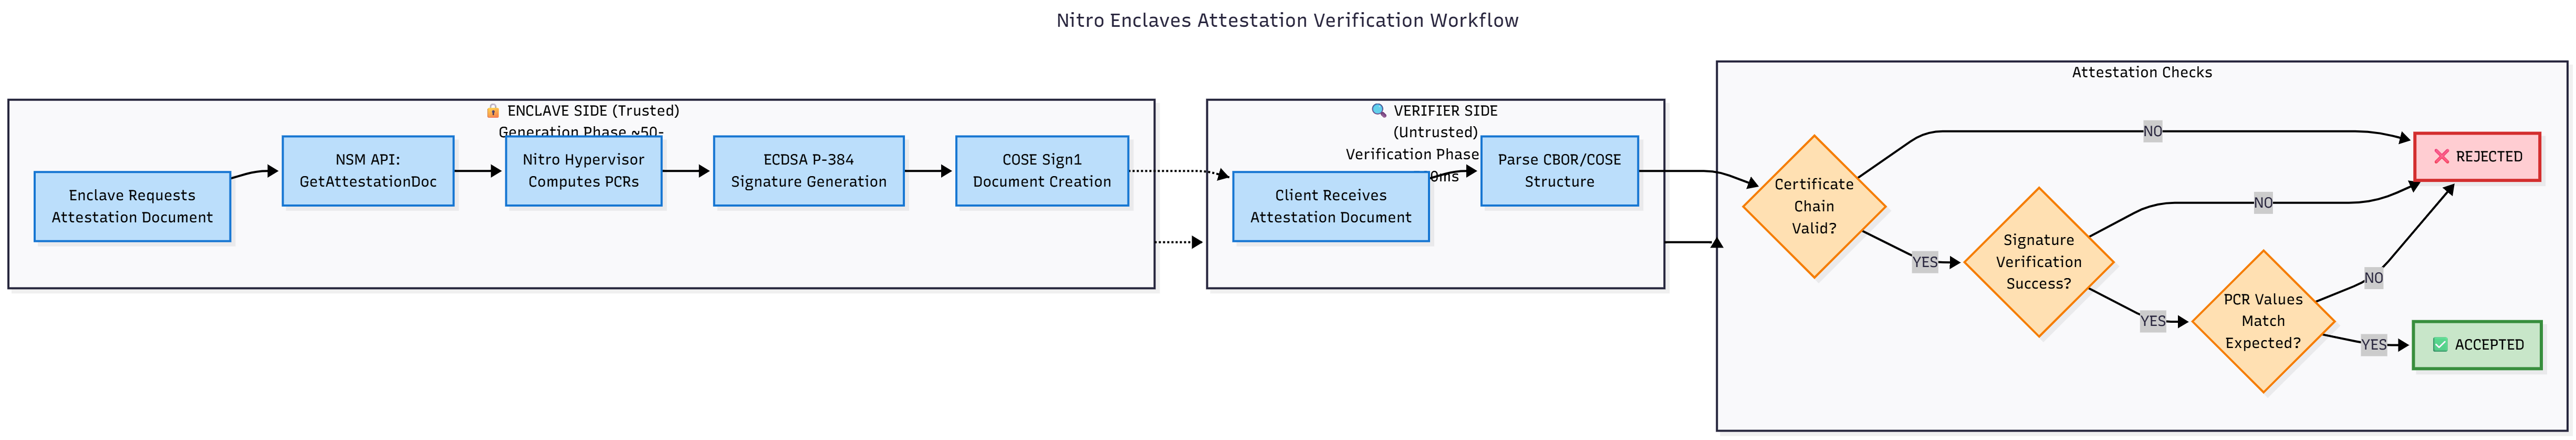
\includegraphics[width=\linewidth]{Figure1.png}
    \caption{Complete attestation document lifecycle from generation within Nitro Enclaves to verification by remote clients. The workflow demonstrates the separation between trusted enclave context and untrusted verification environment.}
    \label{fig:attestation_lifecycle}
\end{figure}




Signature generation occurs within the Nitro Hypervisor as part of the attestation document creation process. When an enclave requests attestation through the NSM API, the hypervisor first computes or retrieves the current Platform Configuration Register values reflecting the enclave's measured state. The hypervisor constructs the attestation document payload as a CBOR map containing these measurements along with timestamp, module identifier, certificates, and any optional fields requested by the enclave. This payload is CBOR-encoded to produce a byte string.

The hypervisor then constructs the \texttt{COSE\_Sig\_structure} that will be signed. This structure is a CBOR array containing the text string \texttt{"Signature1"}, the protected headers byte string specifying the \texttt{ES384} algorithm, an empty byte string for external authenticated data, and the attestation payload byte string. The hypervisor CBOR-encodes this \texttt{Sig\_structure} array to produce the canonical bytes that represent the exact data to be signed. These bytes pass through the \texttt{SHA-384} hash function to produce a 48-byte hash digest.

The \texttt{ECDSA} signing operation uses this hash digest as input along with the hypervisor's private key. The private key exists only within the Nitro Hypervisor security module and is never exposed to any software, including the hypervisor itself. The signing operation produces two integer values, \texttt{R} and \texttt{S}, each 48 bytes in length for the \texttt{P-384} curve. These values are concatenated to produce a 96-byte signature blob. The hypervisor constructs the final \texttt{COSE\_Sign1} structure as a CBOR array containing the protected headers byte string, an empty unprotected headers map, the payload byte string, and the signature byte string. This complete structure is CBOR-encoded and returned to the requesting enclave.

Signature verification by remote parties follows the reverse process while incorporating certificate validation to establish trust in the public key. Verifiers first parse the received CBOR data as a \texttt{COSE\_Sign1} structure, extracting the four elements of the array. The protected headers byte string is decoded as CBOR to extract the algorithm identifier, which must be \texttt{ES384} for Nitro Enclaves attestations. The payload byte string and signature byte string are retained for later processing.


The certificate chain validation precedes signature verification because the signature cannot be trusted without establishing that the public key comes from legitimate AWS infrastructure. Verifiers must have an authentic copy of the AWS Nitro Enclaves root certificate obtained from AWS documentation or other trusted sources. This root certificate serves as the trust anchor for the validation process. The verifier constructs a certificate store or validation context containing this root certificate and configures appropriate validation parameters including checking certificate signatures, validating the certificate validity dates, and verifying that certificates have not been revoked.

The certificate bundle from the attestation document is added to the validation context as intermediate certificates. The verifier then validates the enclave certificate from the attestation document against this context. The validation process checks that the certificate chain from enclave certificate through intermediate certificates to the root certificate consists of valid signatures. Each certificate in the chain must be within its validity period, must have appropriate key usage and extended key usage extensions for the operations being performed, and must not appear on certificate revocation lists if the verifier checks revocation status. Only if the complete chain validates successfully does the verifier proceed to signature verification.

The public key is extracted from the validated enclave certificate. For Nitro Enclaves, this public key is an \texttt{ECDSA} key on the \texttt{P-384} curve. The verifier reconstructs the \texttt{\seqsplit{Sig\_structure}} by creating a CBOR array with the context string \texttt{"Signature1"}, the protected headers byte string, an empty external authenticated data byte string, and the payload byte string. This structure is CBOR-encoded identically to how the signer encoded it, producing the to-be-signed bytes. The verifier computes the \texttt{SHA-384} hash of these bytes, producing the hash digest that was signed.


The signature byte string is parsed into the R and S components by splitting the 96 bytes at the midpoint. These values along with the hash digest and public key serve as inputs to the ECDSA verification algorithm. The verification operation computes whether the signature is valid for the given message hash and public key. Cryptographic libraries may require the signature in different formats such as DER encoding rather than raw concatenation, so verifiers must ensure they provide the signature in the format expected by their chosen library. If the signature verification succeeds, the verifier has cryptographic assurance that the payload was signed by a private key corresponding to the public key in the validated certificate, which chains to the AWS root certificate.

After successful signature verification, the verifier parses the payload byte string as CBOR to extract the attestation document contents. The Platform Configuration Register values are extracted from the PCR map and compared against expected values based on the verifier's attestation policy. The timestamp is checked to ensure the attestation is sufficiently recent. Any application-specific fields such as nonces or user data are validated according to protocol requirements. Only if all these checks pass does the verifier accept the attestation as proof that the specified code is running in a genuine Nitro Enclave.

\subsection{Nitro Security Module API}

The Nitro Security Module provides the interface through which enclave applications request attestation documents and perform other security operations. Understanding the NSM API is essential for developing enclave applications that leverage attestation capabilities. The API design balances between providing necessary functionality and maintaining a minimal attack surface through a constrained interface.

The NSM appears within enclaves as a character device at the path /dev/nsm. Applications open this device file using standard POSIX system calls, obtaining a file descriptor that serves as a handle for subsequent operations. Communication with the NSM occurs through ioctl system calls that send request messages and receive response messages. The request and response messages are encoded as CBOR, maintaining consistency with the attestation document format.

The primary NSM operation is GetAttestationDoc, which generates a signed attestation document reflecting the current enclave state. The request message for this operation can include optional fields for user data, nonce, and public key that will be incorporated into the attestation document. Each of these optional fields has a maximum size of 1024 bytes, limiting the amount of application-specific data that can be included. The NSM validates that the request is well-formed and that optional fields do not exceed size limits before processing the request.

When processing an attestation request, the NSM communicates with the Nitro Hypervisor to obtain current Platform Configuration Register values and generate the signed document. This communication occurs through hypervisor interfaces that are not directly accessible to enclave code, ensuring that applications cannot manipulate the attestation process. The hypervisor performs the actual cryptographic operations including signature generation, as it controls the private keys necessary for signing. The complete signed attestation document is returned to the enclave application through the NSM API as a CBOR-encoded byte sequence.

The GetRandom operation provides access to hardware-based random number generation. Enclave applications can request random bytes in specified quantities, receiving cryptographically secure random data generated by the Nitro System. This capability is essential for cryptographic operations within enclaves, enabling generation of session keys, nonces, and other random values without depending on potentially compromised operating system random number generators. The random data comes from hardware entropy sources, providing high-quality randomness suitable for security-critical operations.

The DescribePCR operation allows applications to query the current value of specific Platform Configuration Registers without generating a complete attestation document. This capability enables applications to inspect their own measured state, which may be useful for debugging or implementing application-specific policies. However, the PCR values obtained through this operation are not signed, so they cannot serve as proof to external parties. Applications must use GetAttestationDoc when cryptographic evidence is required.

The ExtendPCR operation enables dynamic measurement by allowing applications to extend Platform Configuration Register values at runtime. The operation takes a PCR index and data to be measured, computes the hash of current PCR value concatenated with the new data, and updates the PCR with this new hash. This extension mechanism allows enclaves to include application state or configuration in measurements beyond the static measurements computed at initialization. Extended PCRs appear in subsequent attestation documents, enabling policies that constrain runtime behavior in addition to initial configuration.

The LockPCR operation prevents further modifications to specific Platform Configuration Registers. After locking, any attempts to extend the PCR will fail. This capability allows applications to freeze measurements after completing critical initialization steps, preventing subsequent code from altering the measured state. Locked PCRs provide assurance to verifiers that the measurements reflect complete initialization rather than partial state. The lock operation is irreversible for the enclave's lifetime, ensuring that once locked, PCRs remain stable.

The LockPCRs operation extends locking to ranges of PCRs simultaneously. Rather than locking individual registers, applications can lock multiple PCRs atomically. This batch operation ensures consistent locking state across related measurements, preventing race conditions where some PCRs are locked while others remain modifiable. The operation is particularly useful when multiple PCRs together represent a security-relevant configuration that should be frozen as a unit.

Error handling in the NSM API uses standard integer return codes to indicate success or various failure conditions. Success returns zero, while errors return positive integers indicating specific problems such as invalid input, buffer sizes too small, or NSM communication failures. Applications must check return codes and handle errors appropriately, as failure to obtain attestation documents or random values could compromise security. Robust error handling includes retry logic for transient failures while failing safely when persistent errors indicate security-relevant problems.

\subsection{AWS Key Management Service Integration}

AWS Key Management Service provides native integration with Nitro Enclaves attestation, enabling enclaves to access cryptographic keys conditioned on verification of their attested state. This integration solves a critical problem in decentralized AI systems where model weights must be encrypted at rest but decrypted for inference within enclaves. Understanding KMS integration patterns is essential for implementing secure key management in enclave-based applications.

KMS condition keys specific to Nitro Enclaves allow key policies to enforce requirements on Platform Configuration Register values. The condition keys include entries for each PCR, enabling policies to restrict key operations to enclaves with specific measured configurations. For example, a key policy can specify that decryption operations require PCR0 to match a particular hash value identifying an authorized enclave image. Multiple PCR conditions can be combined to enforce comprehensive attestation policies that verify kernel version, application code, IAM role, and signing certificate.

The KMS API operations available from enclaves include Decrypt for converting ciphertext to plaintext, GenerateDataKey for creating data encryption keys, and GenerateRandom for obtaining random bytes. When enclaves call these operations, they provide attestation documents as part of the request. KMS validates the attestation documents by verifying signatures, checking certificate chains, and evaluating PCR values against key policies. Only if all validation succeeds does KMS perform the requested operation and return results to the enclave.

The typical workflow for encrypted model deployment involves several stages. Model providers encrypt AI model weights using a data encryption key, then encrypt that data key using a KMS Customer Master Key with policies restricting decryption to authorized enclaves. The encrypted model and encrypted data key are stored in accessible locations such as S3 buckets. When enclaves start, they load the encrypted data key and request KMS decryption, providing an attestation document proving their configuration. KMS validates the attestation and, if policies are satisfied, decrypts the data key. The enclave uses the decrypted data key to decrypt the model weights, loading them into enclave memory for inference. Throughout this process, the model weights exist in plaintext only within the enclave's protected memory.

KMS key policies must carefully specify which PCR values to enforce. Requiring PCR1 ensures that only enclaves using authorized kernel and boot infrastructure can access keys, preventing attacks that modify these components. Requiring PCR2 ensures that only approved application code can decrypt keys, preventing unauthorized inference implementations. Optionally requiring PCR3 constrains which IAM roles can access keys, enabling organizational access control policies. Requiring PCR8 when using signed enclave images ensures that only images signed by authorized parties can access keys, implementing software supply chain controls.

The certificate validity period of three hours creates challenges for long-running enclaves that need to refresh attestation documents periodically. KMS caches validated attestations for limited periods but eventually requires fresh attestations. Applications must implement logic to regenerate attestation documents before expiration and re-establish KMS sessions using refreshed attestations. The automated refresh process should trigger with sufficient lead time before expiration to handle transient failures without causing service disruption.

Error handling for KMS operations requires attention to both KMS-specific errors and attestation validation failures. KMS may reject requests due to invalid policies, missing permissions, or quota limits independent of attestation validity. Attestation validation may fail due to expired certificates, mismatched PCR values, or signature verification problems. Applications must distinguish between these failure modes and handle them appropriately. Persistent attestation failures indicate security policy violations that should cause enclaves to fail safely rather than continuing without key access.

The security model of KMS integration depends on trust in AWS as both the infrastructure provider and the attestation authority. KMS validates attestations using AWS root certificates and relies on AWS infrastructure to protect master keys. This centralized trust model works for many use cases but represents a limitation for applications requiring decentralized trust. Future enhancements could involve multi-party key management where keys require attestations from enclaves on different cloud providers, reducing centralization at the cost of increased complexity.